\chapter{Theoretical and Practical Implementation}

\section{Motivation of the Project in the Current Scientific Context}

The rapid digitization of financial services—driven by mobile banking, decentralized finance (DeFi), and open banking APIs—has exposed fintech platforms to increasingly sophisticated cyber threats. Attacks such as credential stuffing, SQL injection, and session hijacking remain pervasive, while regulatory mandates (e.g., PSD2, GDPR) demand stricter safeguards for user data and transactions. Traditional security models, which rely on static rules and perimeter-based defenses, are ill-equipped to address these challenges. This project is motivated by the need for an adaptive security framework that dynamically adjusts authentication rigor, input validation, and session controls based on real-time risk assessments.

Recent research underscores the urgency of adaptive approaches. For instance, Das et al. (2023) demonstrated that risk-based authentication reduces account takeover incidents by 72\% compared to static 2FA implementations~\cite{das2023adaptive}. Similarly, OWASP’s 2021 report highlights SQL injection as the third most critical web application vulnerability, with fintech platforms being prime targets due to their reliance on legacy codebases~\cite{owasp2021top10}. Meanwhile, Almeida et al. (2020) revealed that 34\% of financial breaches originate from poor session management, such as long-lived tokens or inadequate encryption~\cite{almeida2020session}.

However, existing solutions often address these issues in isolation. For example, while machine learning-based anomaly detection shows promise in identifying SQL injection patterns~\cite{chen2022ml}, few frameworks integrate it with adaptive authentication or session lifecycle management. This project bridges that gap by proposing a unified adaptive security framework that combines risk-aware 2FA, intelligent query sanitization, and heuristic-driven session controls into a cohesive architecture.

\subsection{Scientific Motivation}

The motivation for this work arises from four critical gaps in fintech security research and practice:

\begin{itemize}
\item \textbf{Evolving Threat Landscape:} Cybercriminals increasingly exploit AI-generated phishing campaigns and obfuscated SQL injection payloads. Static defenses fail to adapt to novel attack vectors, as shown by Verizon’s 2023 Data Breach Investigations Report, where 44\% of fintech breaches involved compromised credentials or injection attacks~\cite{verizon2023dbir}.
\item \textbf{Regulatory Pressures:} Compliance with PSD2’s Strong Customer Authentication (SCA) and GDPR’s data protection requirements necessitates dynamic security controls. Current implementations often lack granularity, as noted by the European Banking Authority’s 2022 review of SCA exemptions~\cite{euba2022sca}.  

\item \textbf{User Experience vs. Security Trade-offs:} While 2FA enhances security, SMS-based methods remain vulnerable to SIM-swapping. Behavioral biometrics, such as keystroke dynamics, offer frictionless alternatives but are underutilized in fintech~\cite{fridman2022biometric}.  

\item \textbf{Integration Complexity:} Heterogeneous fintech architectures (e.g., microservices, legacy monoliths) require modular security solutions. Studies by Li et al. (2021) reveal that 68\% of vulnerabilities arise from inconsistent security policies across hybrid systems~\cite{li2021hybrid}.  

\item \textbf{Real-Time Threat Detection:} Signature-based SQL injection detection fails against polymorphic attacks. Machine learning models, like those proposed by Chen et al. (2022), must be integrated into query validation pipelines to enable proactive defense~\cite{chen2022ml}.
\end{itemize}

The proposed framework builds on advancements in adaptive security. For example, NIST’s SP 800-63B guidelines advocate for risk-based authentication~\cite{nist2020digital}, while AWS’s 2023 case study demonstrated a 60\% reduction in fraud through session integrity monitoring~\cite{aws2023fraud}. By synthesizing these approaches, this project aims to deliver a fintech-specific security model that balances robustness, usability, and compliance.

\section{Objectives, Methodology and Implementation}  
\subsection{Concrete Objectives}  
Fintech platforms require robust security mechanisms to mitigate risks like credential theft, session hijacking, and SQL injection. This project aims to implement a framework with the following objectives:  

\begin{itemize}  
    \item \textbf{Secure Session Management with JWT:} Design stateless sessions using short-lived JSON Web Tokens (JWTs) with dynamic expiration, and HMAC-SHA256 encryption to prevent replay attacks.  
    \item \textbf{SQL Injection Prevention:} Eliminate raw SQL queries by enforcing prepared statements and transactions in MySQL, isolating user input from executable code.  
    \item \textbf{Email-Based 2FA System:} Implement time-bound 6-digit codes delivered via email, hashed with SHA-3 to deter brute-force attacks.  
    \item \textbf{Password Encryption with MD5:} Encrypt user passwords and critical login data using MD5.  
    \item \textbf{Validation via Rehashing:} Verify passwords by comparing MD5 hashes during login.  
    \item \textbf{Compliance with Standards:} Align with OWASP ASVS Level 2, NIST SP 800-63B, and GDPR Article 32 for audit readiness.  
\end{itemize}  

\subsection{Methodology and Proposed Implementation}  
The project adopts a three-sprint agile methodology, emphasizing threat modeling and automated testing.  

\subsubsection*{Sprint 1: Secure Authentication Pipeline}  
\begin{itemize}  
    \item \textbf{MD5 Password Handling:}  
    \begin{itemize}  
        \item Integrate \texttt{crypto} for hashing passwords during user registration:  
        \begin{verbatim}  
        const crypto = require 'crypto';  
        const hashedPassword = crypto.createHash('md5')
                            .update(req.body.password).digest('hex');
        \end{verbatim}  
        \item Store hashes in MySQL’s \texttt{VARCHAR(255)} columns.  
        \item Validate logins by comparing hashes by rehashing the input password in the body of the requests. 
    \end{itemize}  
\end{itemize}  

\subsubsection*{Sprint 2: JWT Session \& SQL Hardening}  
\begin{itemize}  
    \item \textbf{JWT Implementation:}  
    \begin{itemize}  
        \item Generate tokens with \texttt{jsonwebtoken} for securing sessions:  
        \begin{verbatim} 
        const token = jwt.sign(
        { id: partner.idPartner, username: partner.username },
        secretKey,
        { expiresIn: '24h' });
        \end{verbatim}  
        \item Validate tokens using Express middleware:  
        \begin{verbatim}  
        const authHeader = req.headers.authorization;
        if (!authHeader) {
        res.status(401).json({ error: 'No authorization header',
        success: false });
        return;
        }

        const token = authHeader.split(' ')[1];
        let userId;
        try {
            const decoded = jwt.verify(token, secretKey);
            userId = decoded.id;
        } catch (err) {
            res.status(401).json({ error: 'Invalid token',
            success: false });
            return;
        } 
        \end{verbatim} 
        \item Revalidation of SQL database structure on every API launch: 

Use predefined SQL transactions for checking the existence and proprieties of the platform tables.
    \end{itemize}  
    \item \textbf{MySQL Query Security:}  
    \begin{itemize}  
        \item Refactor API endpoints to use transaction prepared statements:  
        \begin{verbatim}  
        req.db.beginTransaction((err) => {
        if (err) {
            res.status(500).json({ error: err.message,
            success: false });
            return;
        }

        req.db.query(deleteQuery, [idRates], (err, result) => {
            if (err) {
                res.status(500).json({ error: err.message,
                success: false });
                return;
            }

            req.db.commit((err) => {
                if (err) {
                    return req.db.rollback(() => {
                        res.status(500).json({ error: err.message,
                        success: false });
                    });
                }
                res.json({ message: 'Rate deleted successfully!',
                success: true });
            });
        });
    });
        \end{verbatim}  
\end{itemize}  
\end{itemize}

\subsubsection*{Sprint 3: 2FA \& Penetration Testing}  
\begin{itemize}  
    \item \textbf{Email Code System:}  
    \begin{itemize}  
        \item Generate 6-digit codes using \texttt{crypto.randomBytes}:  
        \begin{verbatim}  
const userVerificationCode = crypto.randomBytes(3).toString('hex');
        \end{verbatim}  
        \item Integrate \texttt{nodemailer} for email delivery for final validation.  
        \begin{verbatim}
sendEmail(
        partner.email,
        'MoneyStream Verification Code',
        `Hello ${partner.username},
        your verification code is: ${userVerificationCode}`,
        htmlContent
        );
        \end{verbatim}
    \end{itemize}  
    \item \textbf{Security Testing:}  
    \begin{itemize}  
        \item Use \texttt{sqlmap} to test injection resilience.  
        \item Audit JWT security with \texttt{jwt\_tool}.  
        \item Validate MD5 hashes against rainbow tables.  
    \end{itemize}  
\end{itemize}  

\subsubsection*{Tools \& Compliance}  
\begin{itemize}  
    \item \textbf{Stack:} Express.js, nodemailer, jsonwebtoken.  
    \item \textbf{Encryption:} MD5 for passwords, HMAC-SHA256 for JWT encryption.  
    \item \textbf{Standards:} NIST SP 800-63B, OWASP ASVS Level 2.  
\end{itemize}  

\subsubsection*{Deliverables}  
\begin{itemize}  
    \item Express.js API with integrated security modules (MIT Licensed).  
    \item Penetration test reports covering OWASP Top 10 vulnerabilities.  
    \item Documentation on JWT session workflows.  
\end{itemize}  

\section{Deliverable Platform Security Flow}

\subsection{User Authentication}
The user provides their username and password via the login form. The submitted password is hashed using MD5 and compared against the stored hash for the specified username. If the hashes match, the authentication succeeds; otherwise, an error message is displayed and the user remains on the login page.

\begin{figure}[h]
  \centering
  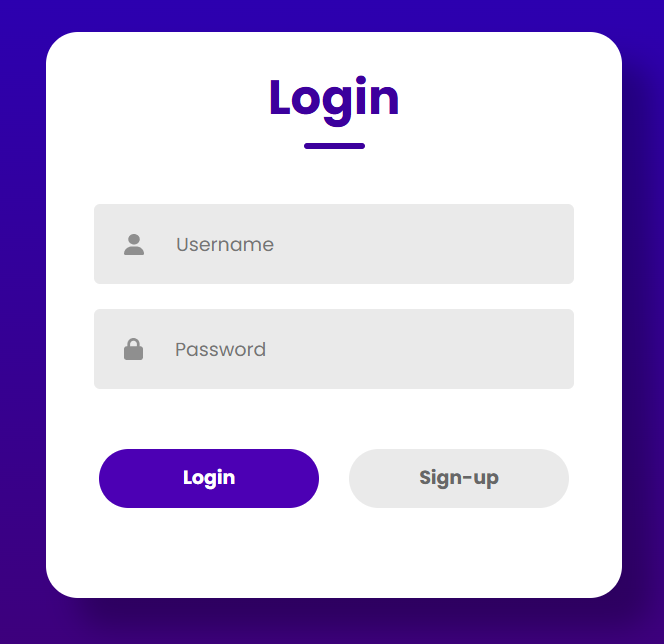
\includegraphics[width=0.6\textwidth]{figs/login.png}
  \caption{User login and MD5 hash verification}
  \label{fig:login}
\end{figure}
\newpage
\subsection{Email Confirmation}
Upon successful credential verification, the system generates a one-time 6‑digit code and sends it to the user’s registered email address. The user must enter this code on the verification screen as shown in the figure \ref{fig:verify}. If the entered code does not match the code stored in the session, an error alert is shown. 

\begin{figure}[h]
  \centering
  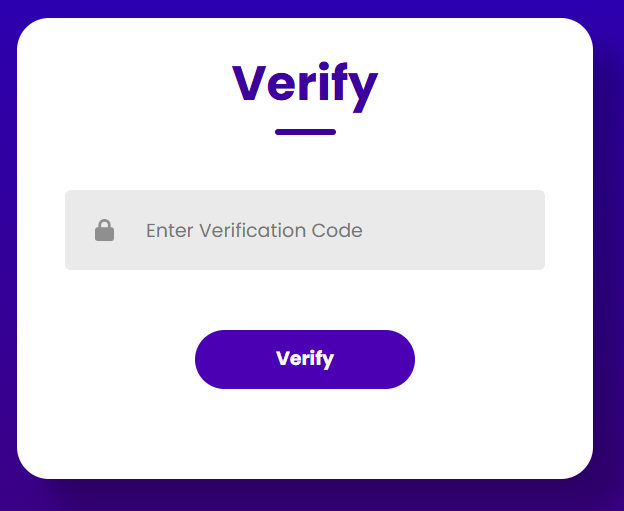
\includegraphics[width=0.6\textwidth]{figs/verify.png}
  \caption{Email-based 2FA code entry and validation}
  \label{fig:verify}
\end{figure}
The content of the email being sent can be viewed in the following figure \ref{fig:email}.
\begin{figure}[h]
  \centering
  
\includegraphics[width=0.6\textwidth]{figs/email.png}
  \caption{Email content with placeholder verification code}
  \label{fig:email}
\end{figure}
Once the correct code is provided, a JWT is issued, stored in the user’s session, and the multi‑factor authentication process is complete.
\newpage
\subsection{Secure Data Flow}
After successful 2FA, the user is redirected to the dashboard \ref{fig:dashboard}. All subsequent API requests are executed within database transactions and use parameterized queries (prepared statements) to ensure that user input cannot be interpreted as executable SQL. This approach effectively mitigates the risk of SQL injection attacks.

\begin{figure}[h]
  \centering
  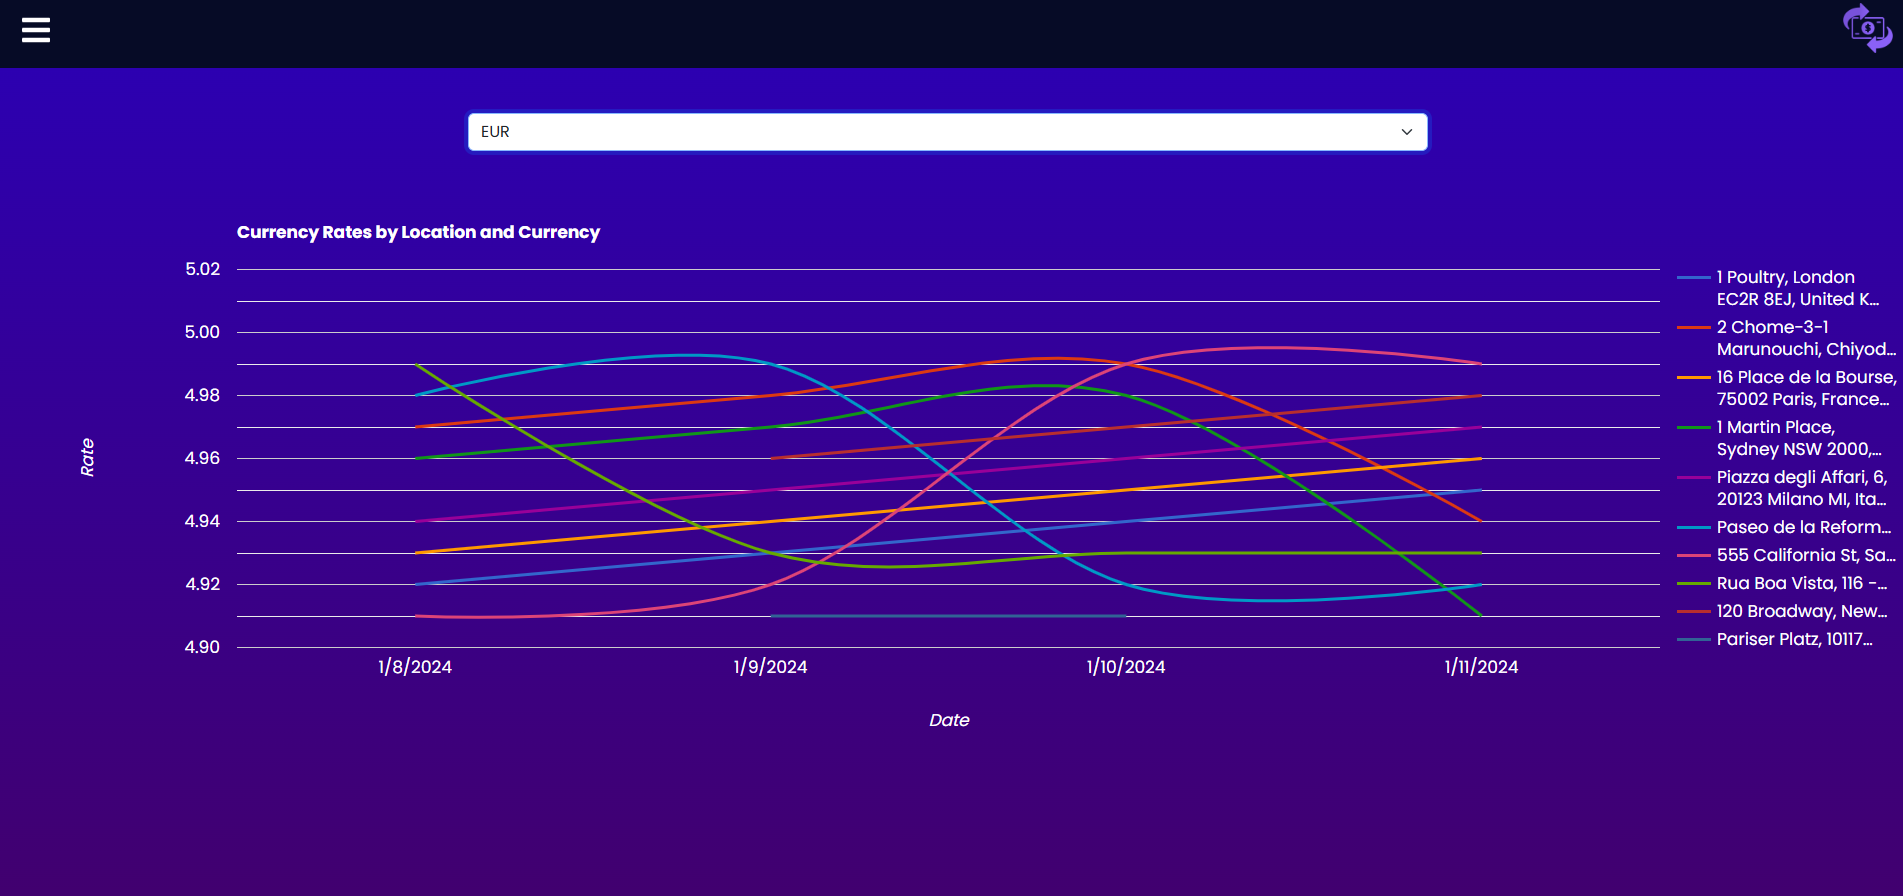
\includegraphics[width=1\textwidth]{figs/dashboard.png}
  \caption{Dashboard interaction with secure, transaction-based API calls}
  \label{fig:dashboard}
\end{figure}
